\begin{figure}[t]
    \centering
    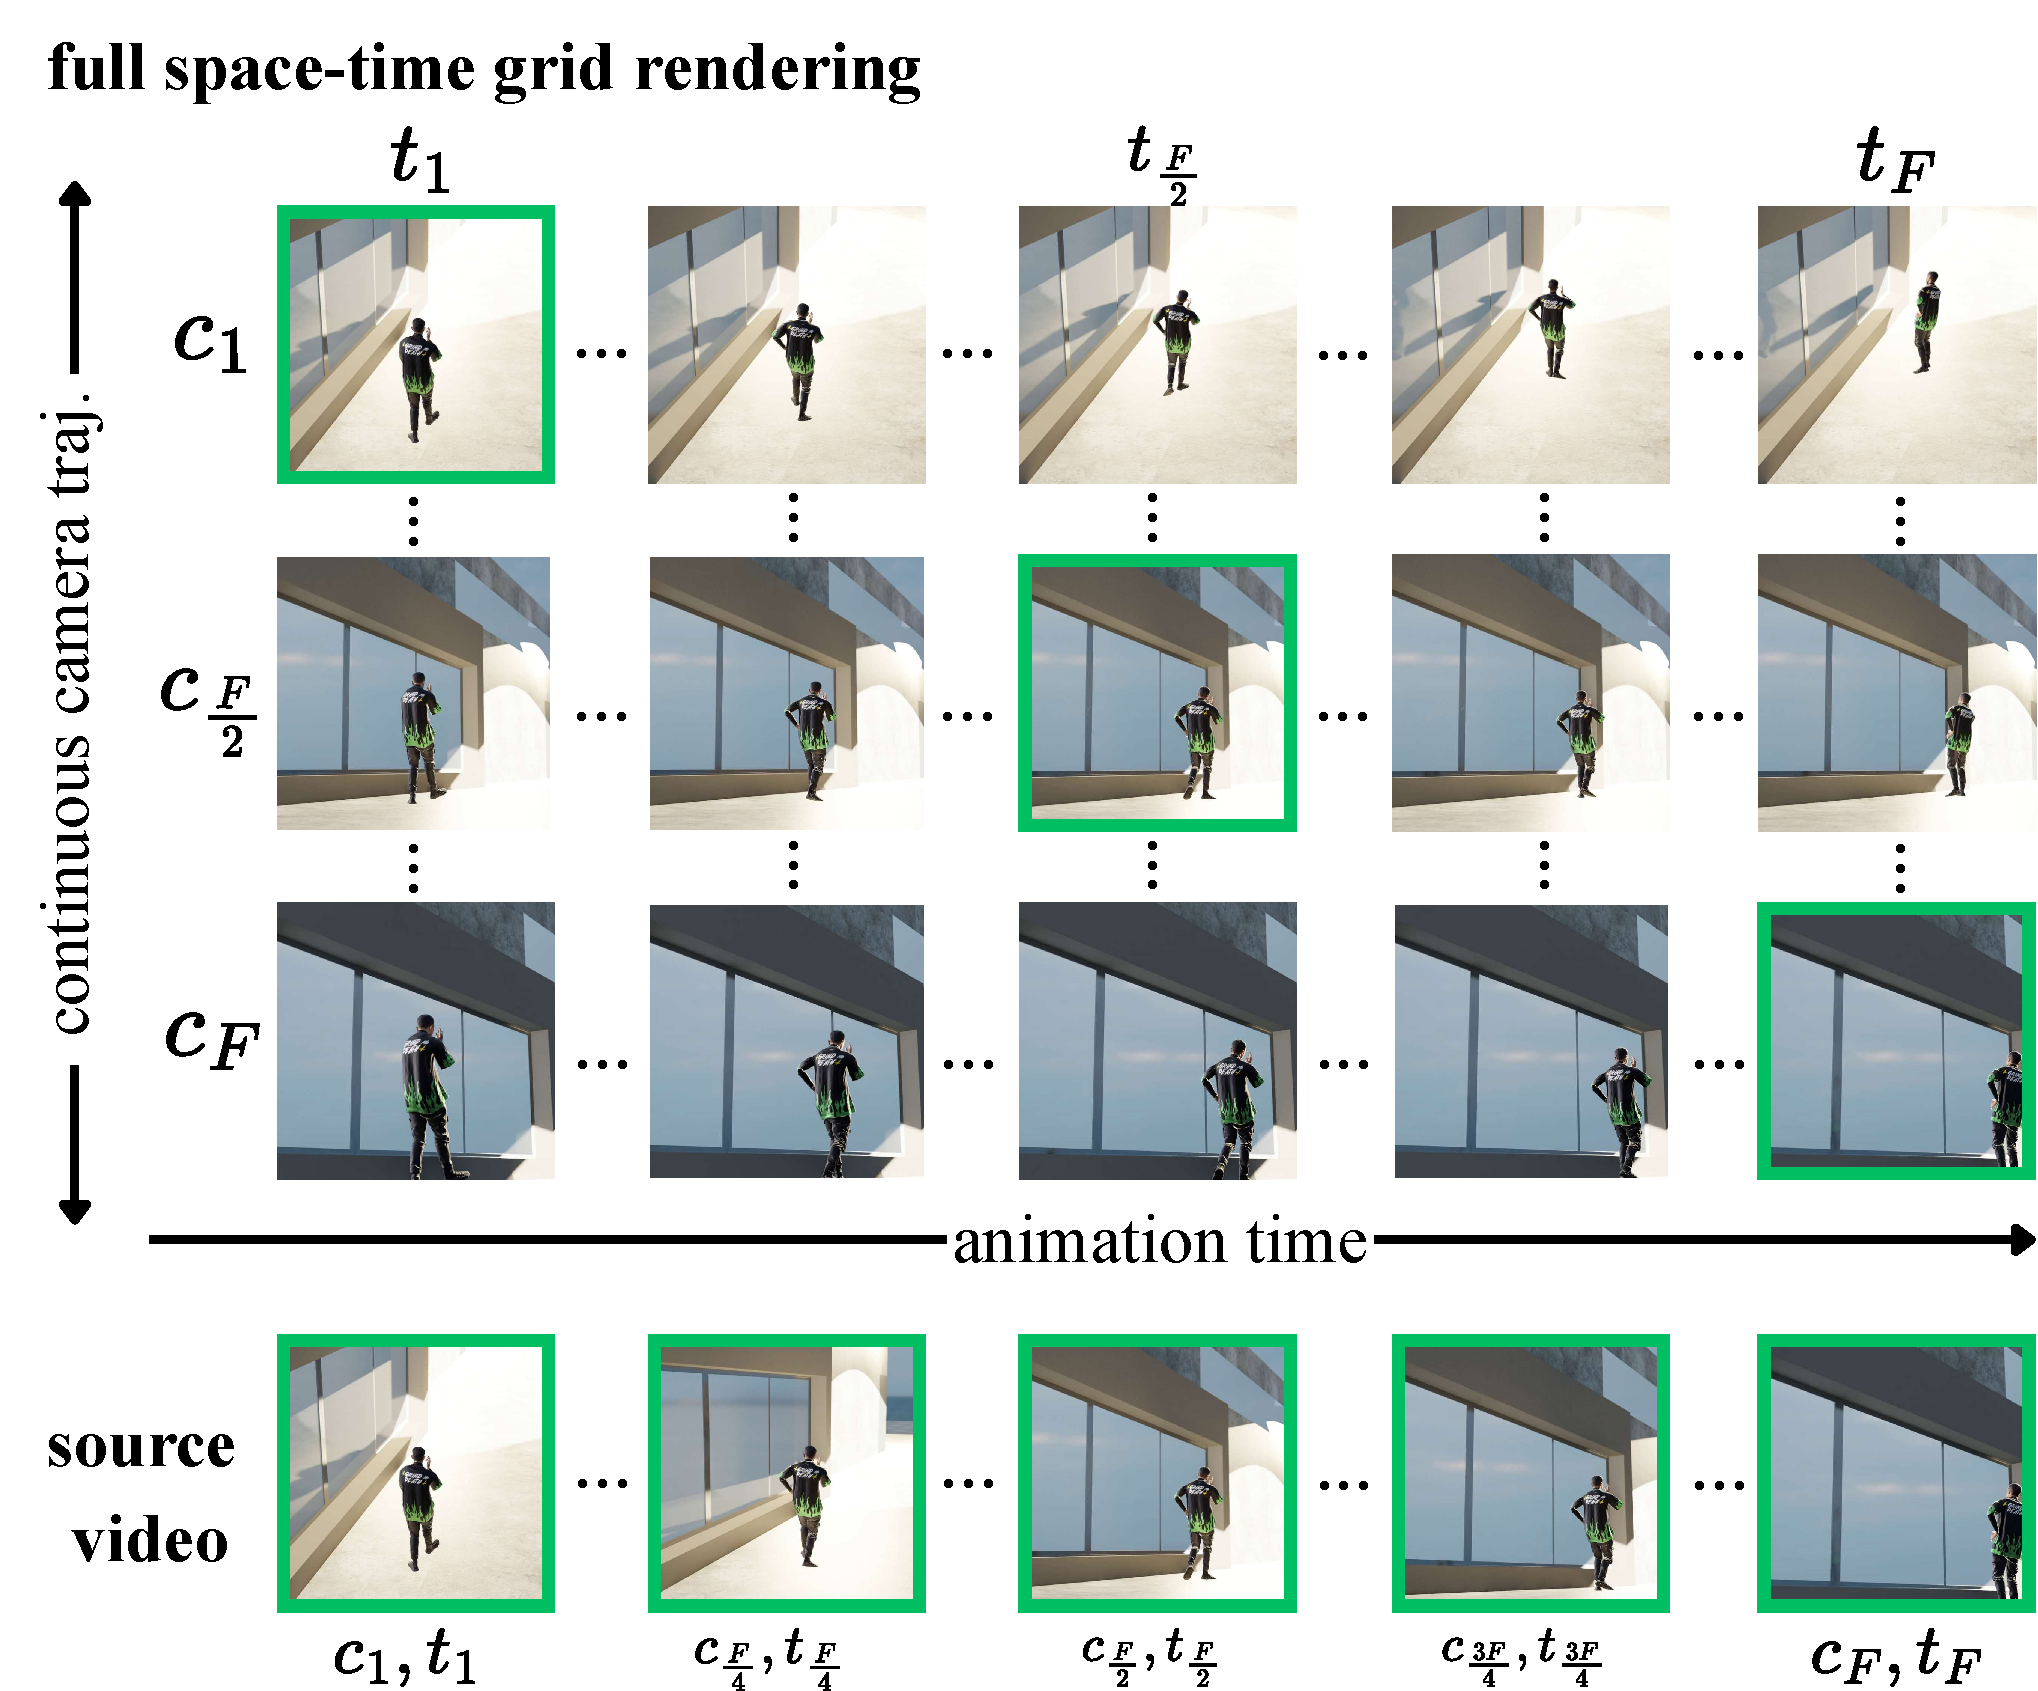
\includegraphics[width=\columnwidth,trim={0 0 0 3mm},clip]{figures/src_files/dataset.pdf}
    \caption{
    \textbf{\textit{\nameDataset} dataset visualization}. (Top) A space-time grid defined by a camera trajectory $\camera=[c_1,...,c_F]$ and animation status $\animatime=[t_1,...,t_F]$. \nameDataset renders images for all $(c,t)$ pairs, covering the full grid for learning disentangled spatial and temporal control. Any two sampled  sequences of $\numf$ frames from the grid can form a source-target pair. (Bottom) One typical choice of source videos is taking the diagonal cells in     green. }
    \label{fig:dataset_blender}
    \vspace{-0.3cm}
\end{figure}
